   This chapter will give an overview to the ways this project was managed internally, as well as by the supervisors. It includes a detailed introduction to the Kanban - management tool, followed by complementary techniques used by the team to further improve the working process.
    \section{Kanban}
For internal management of the team, based on the suggestions of our industry partners, it was decided to use an Agile product management technique - Kanban. It emphasizes on a continuous delivery mindset, trying not to overburden the development team. Like other Agile techniques, it was designed to facilitate communication and division of work inside the team, while giving live updates so each member can keep up with the process. The simple and intuitive structure helps the team work in a more efficient way.
% Marius: More efficient than what?
        \subsection{Principles}
        Kanban is build by respecting the following 3 principles:
            \begin{enumerate}
  \item \textbf{Visualization}: Kanban uses mechanisms organised in a Kanban board. The board, by presenting all the tasks at once, in an easy to grasp manner, gives the developer a better understanding of the context, thus facilitating the workflow.
  \item \textbf{Limited amount of work}: because the number of tasks are limited from a week to another (as well as the number of cards stored in production) the team does not feel overburdened with work, and is not pressured to deliver something by sacrificing on the quality aspect.
  \item \textbf{Continuous flow}: when a member is done with his/her tasks, he/she can just move forward with the work process by picking up the next tasks (placed on the top of the stack). This way nobody sits around waiting to be designated with work, thus ensuring a continuous workflow.
\end{enumerate}
        \subsection{Benefits}
        Taking in consideration the above mentioned information, it is easy to identify the way this project management method can improve the delivery process of a product, following are a couple of its advantages: 
            \begin{enumerate}
                \item \textit{Kanban methodology utilizes short working cycles.} In the case of this project the cycle was limited at one week (with an exception during the winter break).  This 1 week cycles ensured a continuous delivery process, where the industry partners had the opportunity to keep the team in check, by introducing new features/corrections in the process.
                \item \textit{Kanban is very responsive to change and feedback.} As mentioned above, thanks to a short cycle, the BMW representatives had the opportunity to introduce change in an utile time, by coming up with new features or scenarios, as well as feedback to improve or correct the direction of the project.
                \item \textit{Kanban removes time wasting activities.} While popular management techniques require a series of mandatory daily meetings and discussions, Kanban eliminates this type of time wasting activities. Meetings were organized once a week or on team’s request, in cases of confusion or identification of impediments of the working process that should be discussed and solved at team level.
            \end{enumerate}
        \subsection{Roles}
Given the Kanban approach, it does not have well predefined roles. It suggests to start from the structure of your team, and current management, and to evolve it as seen necessary, taken in consideration the specific of the methodology.
As the team had no previous experience working together, it decided to have a Project Manager that would facilitate the communication between them and the supervisors, as well as take care of organizational issues.
The project manager’s responsibilities are:
            \begin{itemize}
              \item Managing the Kanban board (in Trello) which means writing down the tasks, assigning responsible people, adding labels, deadlines (if necessary), updating the progress, and cleaning up the board by periodically archiving the old cards.
              \item Managing other means of communication, like Slack, by organizing specific channels, setting up notifications and reminders.
              \item Setting up and managing meetings, making sure they are productive and that the team is up to date with project’s progress.
              \item Being the spokesperson for the team, mediating the communication with the supervisors.
            \end{itemize}
        \subsection{Kanban board}
As already mentioned above, Kanban uses a board as it’s main management tool. A Kanban board is designed to help visualise the workflow. A typical board can be broken down into the following elements:
            \begin{enumerate}
                \item Cards or Visual Signals 
                \item Columns
                \item Work in Progress (WIP) Limits
            \end{enumerate}
The visual signals are usually the tasks that are written on stickies, in the case of a physical board, or on cards, in the case of software based boards. Each card encapsulates one user story, and all the user stories should require an equal or at least close enough effort. Once written down and attached to the board, these visual signals help the team, as well as other stakeholders, understand the product development.
Columns represent different production stages that an user story can be in. All these stages together compose the workflow. The columns can be as simple as “To do”, “In progress” and “Done”, to more complicated stages, depending on the complexity of the development process.
Work in Progress Limits are the maximum number of cards that can be placed in a certain column at a certain period of time. This is done in order to limit the team’s ability to commit to too much work in a short period of time.
                \subsubsection{Trello as a Kanban board}
For the project, the team decided, following the supervisors’ suggestion, to use a digital board. This allows it not to share a physical space (like an office), and to work remotely and asynchronously. Trello is one of the simplest and easiest way to mimic a Kanban board by allowing the users to create lists, that mimic the columns, and cards that represent user stories.

For this project, it was decided to create the following workflow structure:
    \begin{itemize}
        \item Backlog - aggregates all user stories
        \item Breakdown (Doing and Done)- splits up user stories in smaller units of work
        \item Implementation (Doing and Done) - indicates what cards are currently in work
        \item Validation (Doing and Done)- tests the finished user stories against the definition-of-done.
    \end{itemize}

    \begin{figure}[h]
        \centering
        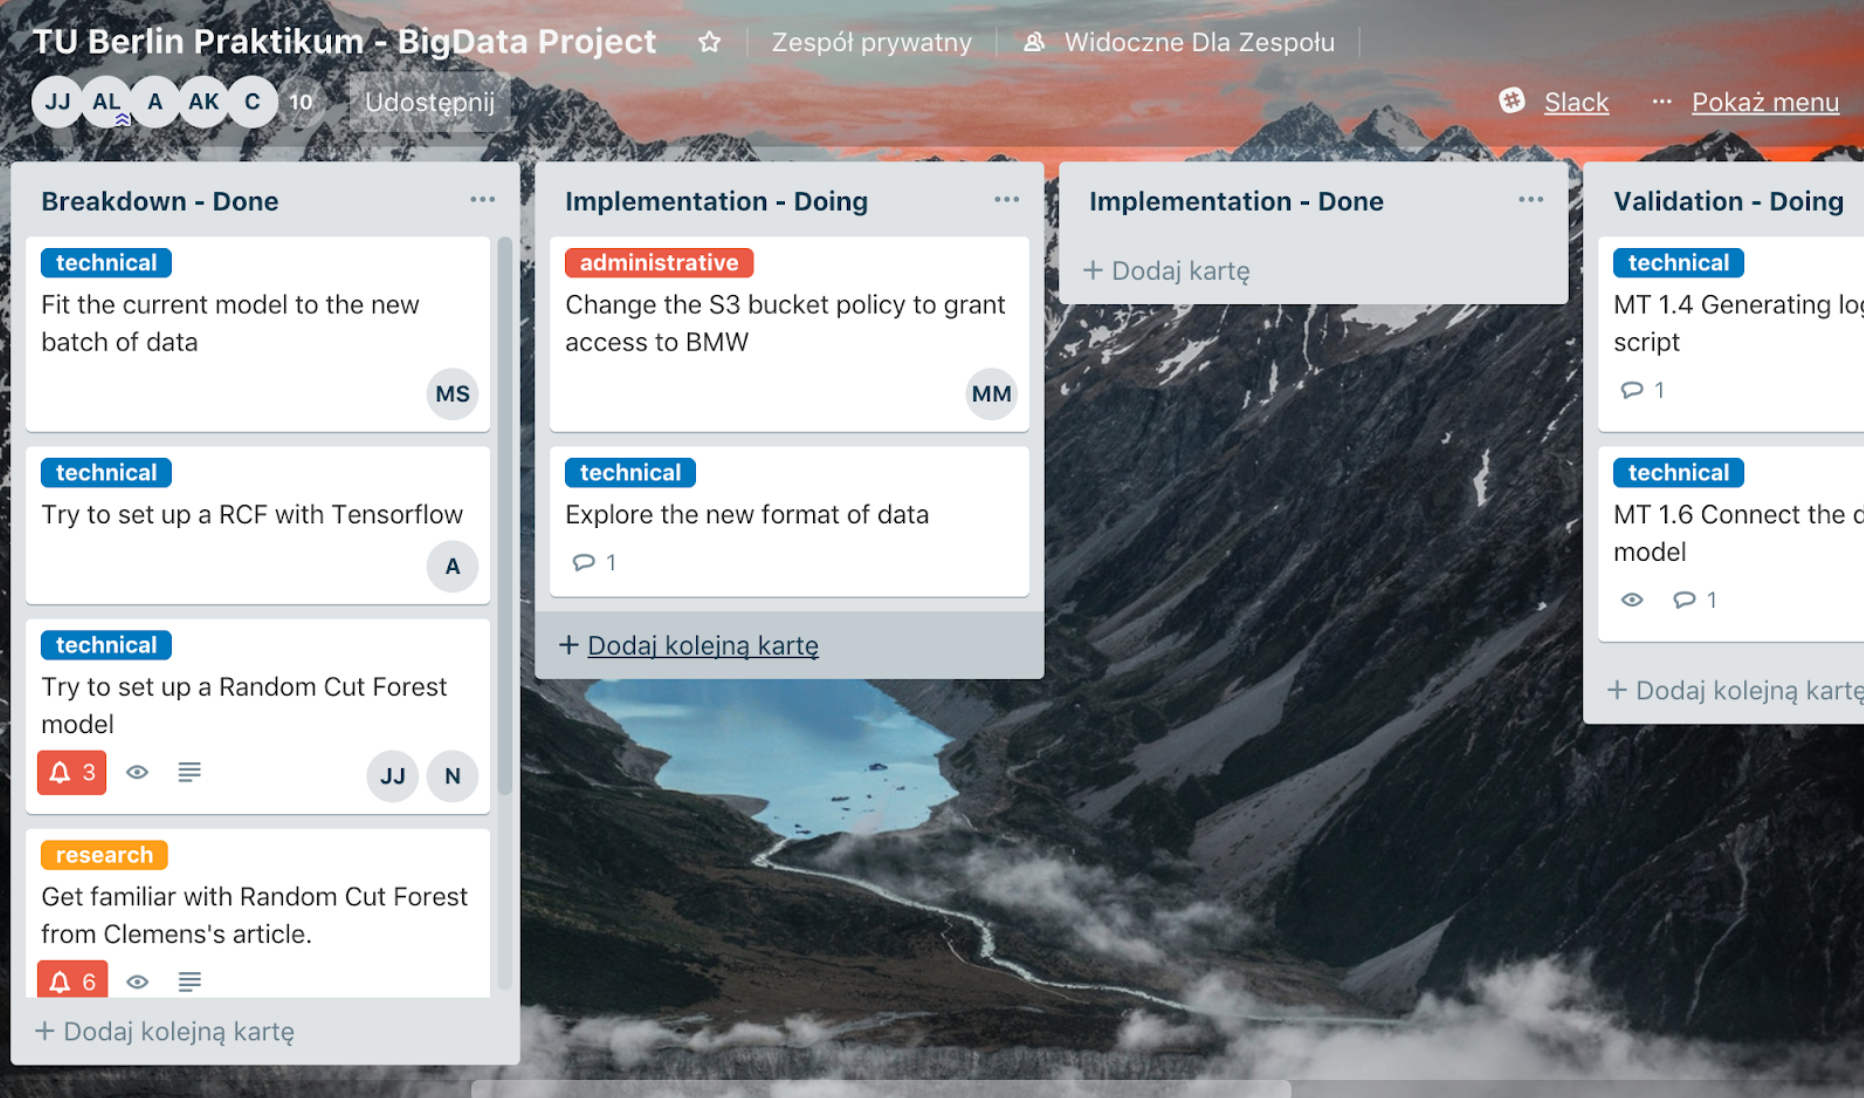
\includegraphics[width=1\textwidth]{images/trello.png}
        \caption{Big Data Analytics Trello board }
        \label{fig:trello_board_1}
    \end{figure}
    
After setting up the above mentioned columns, a user can start adding cards/user stories to the backlog. As seen in figure \ref{fig:trello_board_1}, Trello allows an user to add a title, a description (to detail the card), attachments, comments, due dates, responsible members and labels to a card.
It's worth noting, that for this project, the team used the board not just for programming related tasks. The Trello board was used for managing all project related assignments, for the purpose of registering each week's work.
\begin{figure}
    \centering
    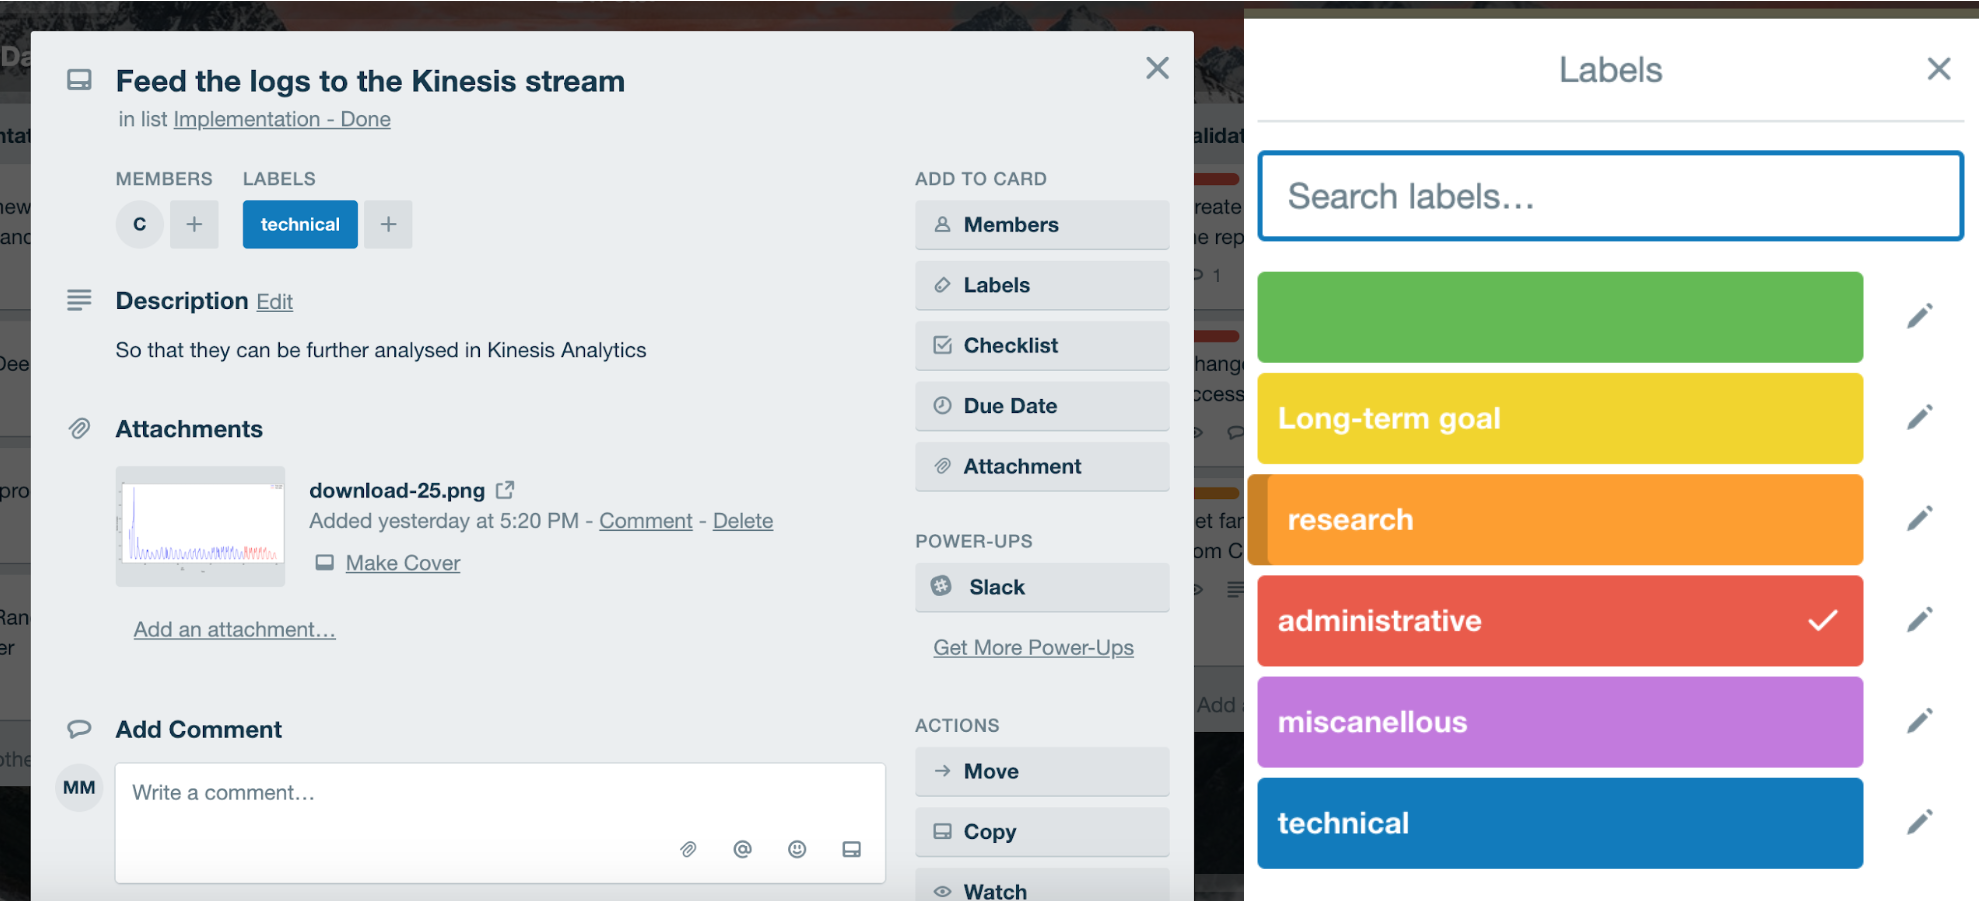
\includegraphics[width=1\textwidth]{images/card-view.png}
    \caption{Trello board card view with labeling details }
    \label{fig:fig:trello_board_2}
\end{figure}
In this project, the team used the following series of labels to mark the purposes of the user-story (see \ref{fig:trello_board_2}):
    \begin{itemize}
    \item \textbf{Long-term goal}: indicates that the card is most likely a use case in the project, which should be broken down further into smaller tasks
    \item \textbf{Research}: marks tasks that require the team to look for papers, documentation, solutions to solve certain impediments
    \item \textbf{Administrative}: highlights that a task has a managerial character
    \item \textbf{Technical}: indicates a developer task;
    \item \textbf{Miscellaneous}: used for any other subjects that a task can have, except the ones mentioned above (e.g. creating the presentation or documentation paper)
\end{itemize}
    